
%----------------------------------------------------------------------------------------
%	Settings and packages
%----------------------------------------------------------------------------------------

\documentclass[10pt]{article}

\usepackage{colortbl}
\usepackage{multirow}
\usepackage[table]{xcolor}
\usepackage{ctable}
\usepackage{float}
\usepackage{adjustbox}
\usepackage[landscape,margin=0.25in,legalpaper]{geometry}

\newcommand{\mcn}[2]{\multicolumn{#1}{l}{#2}}	
\newcommand{\mccn}[2]{\multicolumn{#1}{c}{#2}}
\newcommand{\mcl}[1]{\multicolumn{2}{l}{#1}}
\newcommand{\mclg}[1]{\multicolumn{2}{l}{\gr #1}}
\newcommand{\mcc}[1]{\multicolumn{2}{c}{#1}}
\newcommand{\mccg}[1]{\multicolumn{2}{c}{\gr #1}}
\newcommand{\mr}[1]{\multirow{-2}{*}{#1}}
\definecolor{Gray}{gray}{0.90}
\newcommand{\gr}{\cellcolor{Gray}}

\newcommand{\thickline}{\specialrule{.1em}{.05em}{.05em}}

\setlength\parindent{0pt}

% column colours
\newcolumntype{g}{>{\columncolor{Gray}}l}
\newcolumntype{w}{>{\columncolor{white}}l}

%----------------------------------------------------------------------------------------
%	Table
%----------------------------------------------------------------------------------------

\begin{document}

\thispagestyle{empty}
{\bf 2012 Deepwell Cup}
\begin{table}[h!]
  \centering
  \adjustbox{max width=\textwidth}{
    \begin{tabular}{l g g w w g g w w g g w w g g w w g g w w g g w w g g}
        \rowcolor{black}\mcn{27}{\color{white}\bf Round 4: Stanley Cup Finals} \\
        \rowcolor{white}\\
        & \mccg{Alita D} & \mcc{Andre D} & \mccg{Andrew D} & \mcc{Andy H} & \mccg{Charmaine L} & \mcc{David D} & \mccg{Isaiah C} & \mcc{Kollin H} & \mccg{Kyle L} & \mcc{Mark D} & \mccg{Michael D} & \mcc{Nathaniel T} & \mccg{Thomas L}  \\\thickline
&&&&&&&&&&&&&&&&&&&&&&&&&& \\\hline
          New Jersey Devils&&&&&&&&&&&&&&&&&&&&&&&&&&\\
          Los Angeles Kings & \mr{LAK} & \mr{6} & \mr{LAK} & \mr{6} & \mr{LAK} & \mr{5} & \mr{LAK} & \mr{6} & \mr{LAK} & \mr{7} & \mr{LAK} & \mr{6} & \mr{LAK} & \mr{5} & \mr{LAK} & \mr{6} & \mr{} & \mr{6} & \mr{LAK} & \mr{6} & \mr{LAK} & \mr{6} & \mr{NJD} & \mr{7} & \mr{LAK} & \mr{5}\\\hline
          \rowcolor{white}\\
        \rowcolor{black} \mcn{27}{\color{white}\bf Conference Champions} \\
          Eastern & \mclg{NYR} & \mcl{NYR} & \mclg{NYR} & \mcl{PIT} & \mclg{PIT} & \mcl{BOS} & \mclg{BOS} & \mcl{PIT} & \mclg{NYR} & \mcl{PIT} & \mclg{BOS} & \mcl{PIT} & \mclg{PIT}\\
          Western & \mclg{VAN} & \mcl{VAN} & \mclg{VAN} & \mcl{VAN} & \mclg{VAN} & \mcl{VAN} & \mclg{VAN} & \mcl{DET} & \mclg{VAN} & \mcl{VAN} & \mclg{VAN} & \mcl{VAN} & \mclg{VAN}\\
          Stanley Cup & \mclg{VAN} & \mcl{VAN} & \mclg{VAN} & \mcl{PIT} & \mclg{VAN} & \mcl{VAN} & \mclg{VAN} & \mcl{PIT} & \mclg{VAN} & \mcl{VAN} & \mclg{VAN} & \mcl{VAN} & \mclg{VAN}
    \end{tabular}
  }
\end{table}

{\bf Points}\\
\begin{minipage}[t]{12cm}
    \vspace{0pt}
    \begin{tabular}{l l}
        Correct team:	& $7$\\
        Correct series length (regardless of series winner):	& $10$\\
        Stanley Cup champion:	& 25\\
        Stanley Cup runner-up:	& 15\\
    \end{tabular}

    \vspace{0.5cm}
    {\bf Number of picks:}\\
    \begin{tabular}{lc }
        NJD & 1 \\
        LAK & 11 \\
    \end{tabular}
\end{minipage}
%
\begin{minipage}[t]{13cm}
    \vspace{0pt}
    \begin{figure}[H]
        \vspace{-1cm}
        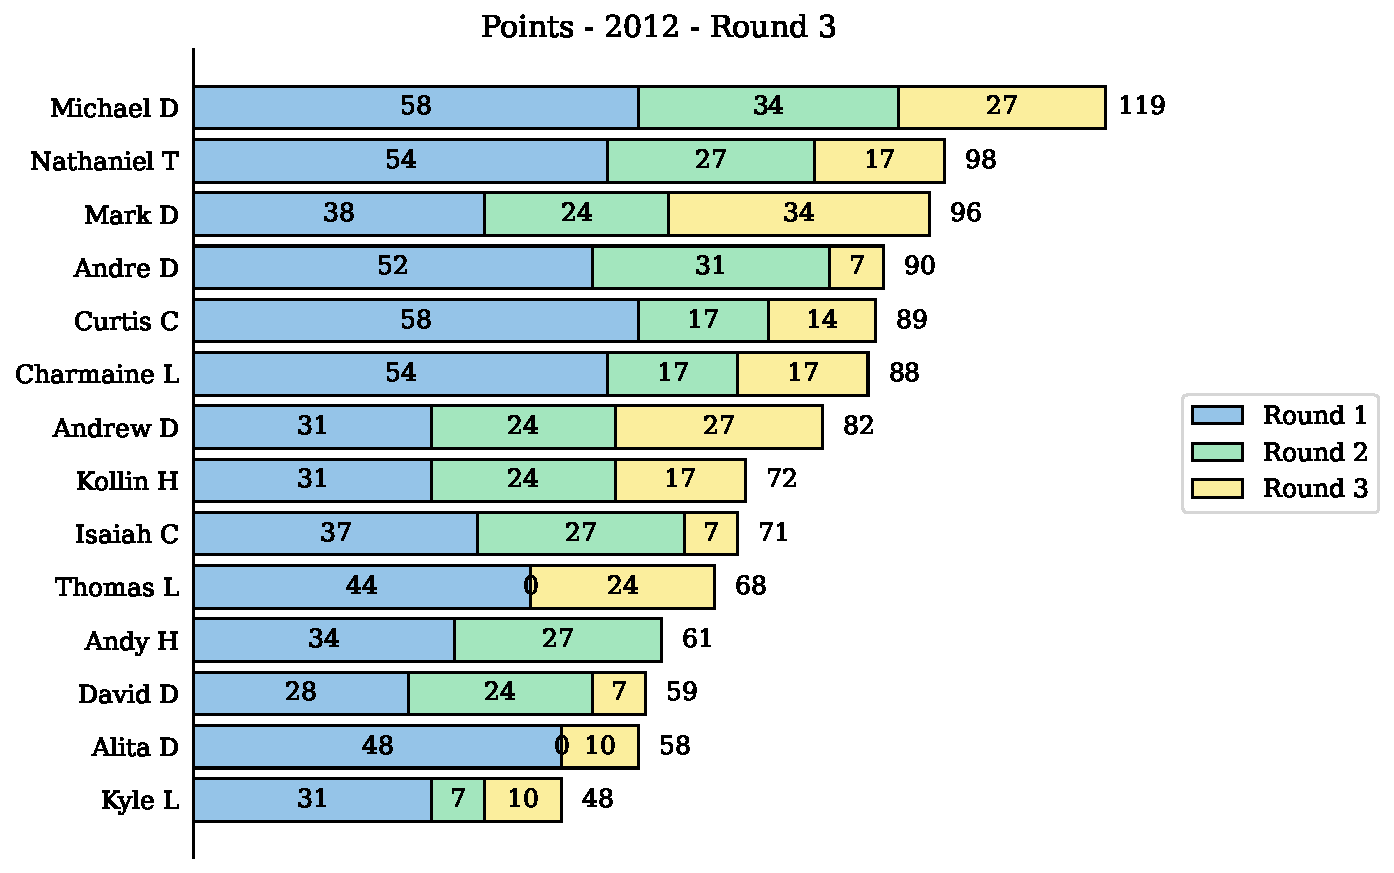
\includegraphics[width=12cm,height=8cm,keepaspectratio]{../../figures/2012/Points-2012-Round3.pdf}
    \end{figure}
\end{minipage}

\end{document}